\section{Fallrad} % vorläufiger Name
	
	Das Fallrad verhält sich wie das Jo-Jo Spielzeug. Lässt man das aufgewickelte Fallrad fallen, bei festgehaltener Schnur, so fällt es langsamer und und wickelt sich nach Abwickeln der Schnur von selbst wieder auf. In diesem Versuch werden die Fallbeschleunigung und das Trägheitsmoment eines Fallrades bestimmt und überprüft, ob die gemessenen und bestimmten Werte mit den aus der Theorie berechneten Werten übereinstimmen. Dazu wird angenommen, dass die aus der Theorie bekannten Formeln den Sachverhalt korrekt beschreiben. Das Ergebnis dieses Versuches stimmt mit diesen (nicht) überein. % TODO 
	
	\subsection{Methoden}
		
		\subsubsection{Aufbau}
		
			\begin{figure}[ht]
				\centering
				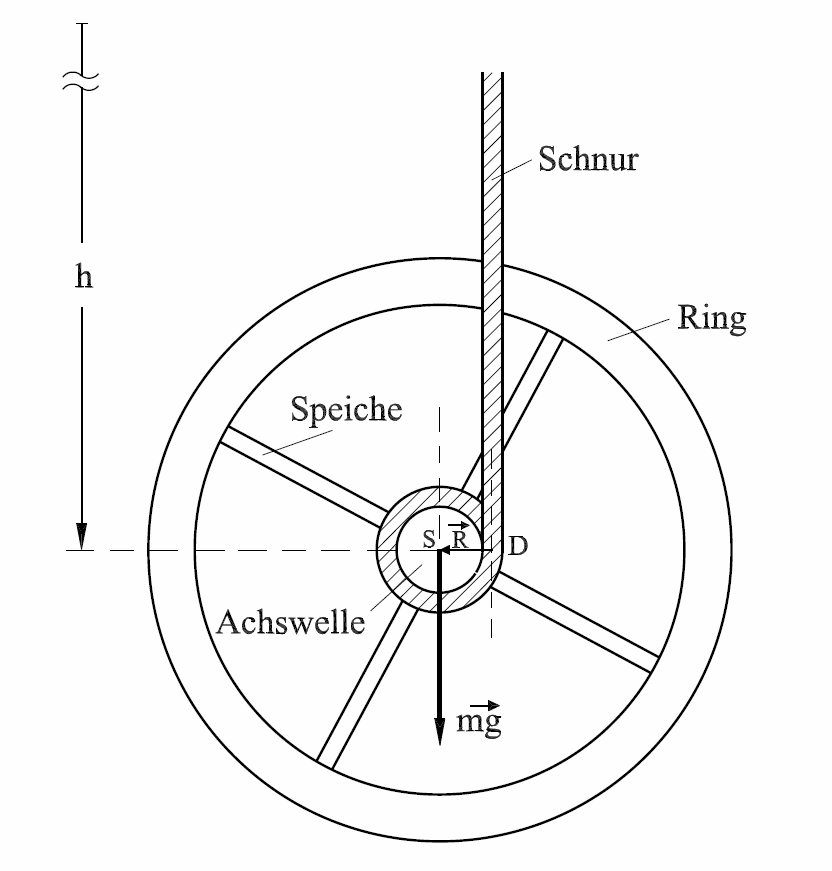
\includegraphics[width=0.7\textwidth]{fallrad_skizze.png}
				\caption{Versuchsskizze: Seitenansicht des Fallrades}
				\label{fig:FallradSkizze}	
			\end{figure}
			Es wird der in Abb. \ref{fig:FallradSkizze} dargestellte Aufbau betrachtet. 
			Das Fallrad besteht aus einem Ring, in dessen Mittelpunkt sich die Achse befindet, um welche die Bewegung durchgeführt wird. Mit Hilfe von vier Speichen ist der Ring mit der Achse verbunden. Zur Vereinfachung wird angenommen, dass es sich hierbei um zwei senkrecht zueinander liegende Zylinder handelt, die in ihren Mittelpunkten mit der Achse verbunden sind. 
			Die Achse liegt mittig in dem Ring, sodass die Schnur auf beiden Seiten mit dem gleichen Abstand von dem Ring angebracht werden kann (vgl. \ref{fig:FallradFrontal}). 
			\begin{figure}[ht]
				\centering
				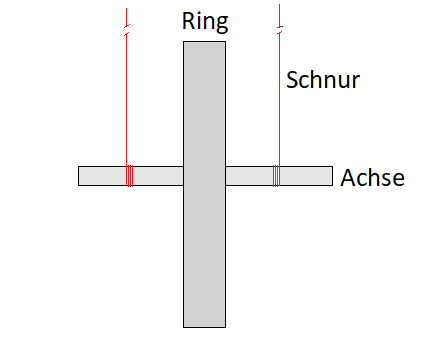
\includegraphics[width=0.6\textwidth]{fallrad_frontal.png}
				\caption{Frontalansicht des Fallrades}
				\label{fig:FallradFrontal}	
			\end{figure}
			In der Ruhelage liegen keine Wicklungen der Schnur auf der Achse vor. Die Größe $h$ gibt die Höhe des Fallrades, als Abstand von der Ruhelage, an. 
		
		\subsubsection{Durchführung}
			
			Mit einer Stoppuhr wird die Zeit gemessen, die das Fallrad benötigt bis es bei $h=0$ angekommen ist. Dies wird für verschiedene Starthöhen durchgeführt um die Fallbeschleunigung $g^{*}$ zu bestimmen. Dafür ist es wichtig darauf zu achten, dass die Schnur sich bei dem Aufwickeln nicht auf sich selber, sondern nur auf der Achse wickelt, damit sich der Abrollradius nicht verändert.
			
			Zur Bestimmung des Trägheitsmoments werden die Maße des Fallrads mit Hilfe einer Schiebelehre gemessen und die Masse gewägt.			
			
		\subsubsection{Unsicherheiten}
			
			Im Allgemeinen dient zur Berechnung der Unsicherheiten für die gemessenen und ermittelten Werte folgende Formel: 
			\begin{equation*}
				u(s) = \pm \sqrt{\sum_{k=0}^{N}\left( \frac{\partial f}{\partial x_i}u(x_i)\right) ^2}. \label{eq:kombUnsicherheit}
			\end{equation*}
			Für die Messunsicherheit der Stoppuhr wird aufgrund der Digitalanzeige eine Rechtecksverteilung verwendet und diese dann mit der Unsicherheit für die Reaktionszeit kombiniert. Die Schiebelehre besitzt eine Messgenauigkeit von \SI{0,02}{\mm}, da sich so genau jedoch nicht ablesen lässt, wird eine Dreicksverteilung mit  \SI{0,04}{\mm} verwendet.
			Die Berechnung der Unsicherheiten liegt im Anhang vor, da diese für einige Größen umfangreicher ist.
			
	\subsection{Messung}
	
		\subsubsection{Aufnahme der Messwerte}
	
		\subsubsection{Datenanalyse}	

	\subsection{Diskussion}
		
	\subsection{Schlussfolgerung}
	